\section{Expanding the Model for Effectiveness}

The larger evaporative cooler, Option C, was the unique minimax choice at all 12 venues. It had the lowest modeled residual discomfort outright in 28 of 36 cases and tied for the lowest in the other eight.

We measured residual discomfort as SET degree-hours above 26\ensuremath{^{\circ}\mathrm{C}} for the reference person. For a one-hour case, a SET of 30\ensuremath{^{\circ}\mathrm{C}} gives four degree-hours of residual discomfort. Regret is the option's residual discomfort minus the smallest residual discomfort among feasible options in the same case.

For each venue, we took the maximum regret of each option over the three weather scenarios and selected the feasible option with the smallest maximum. We included the no-device baseline and evaluated the baseline model with budget, electricity, and water caps disabled.

\begin{figure}[H]
    \centering
    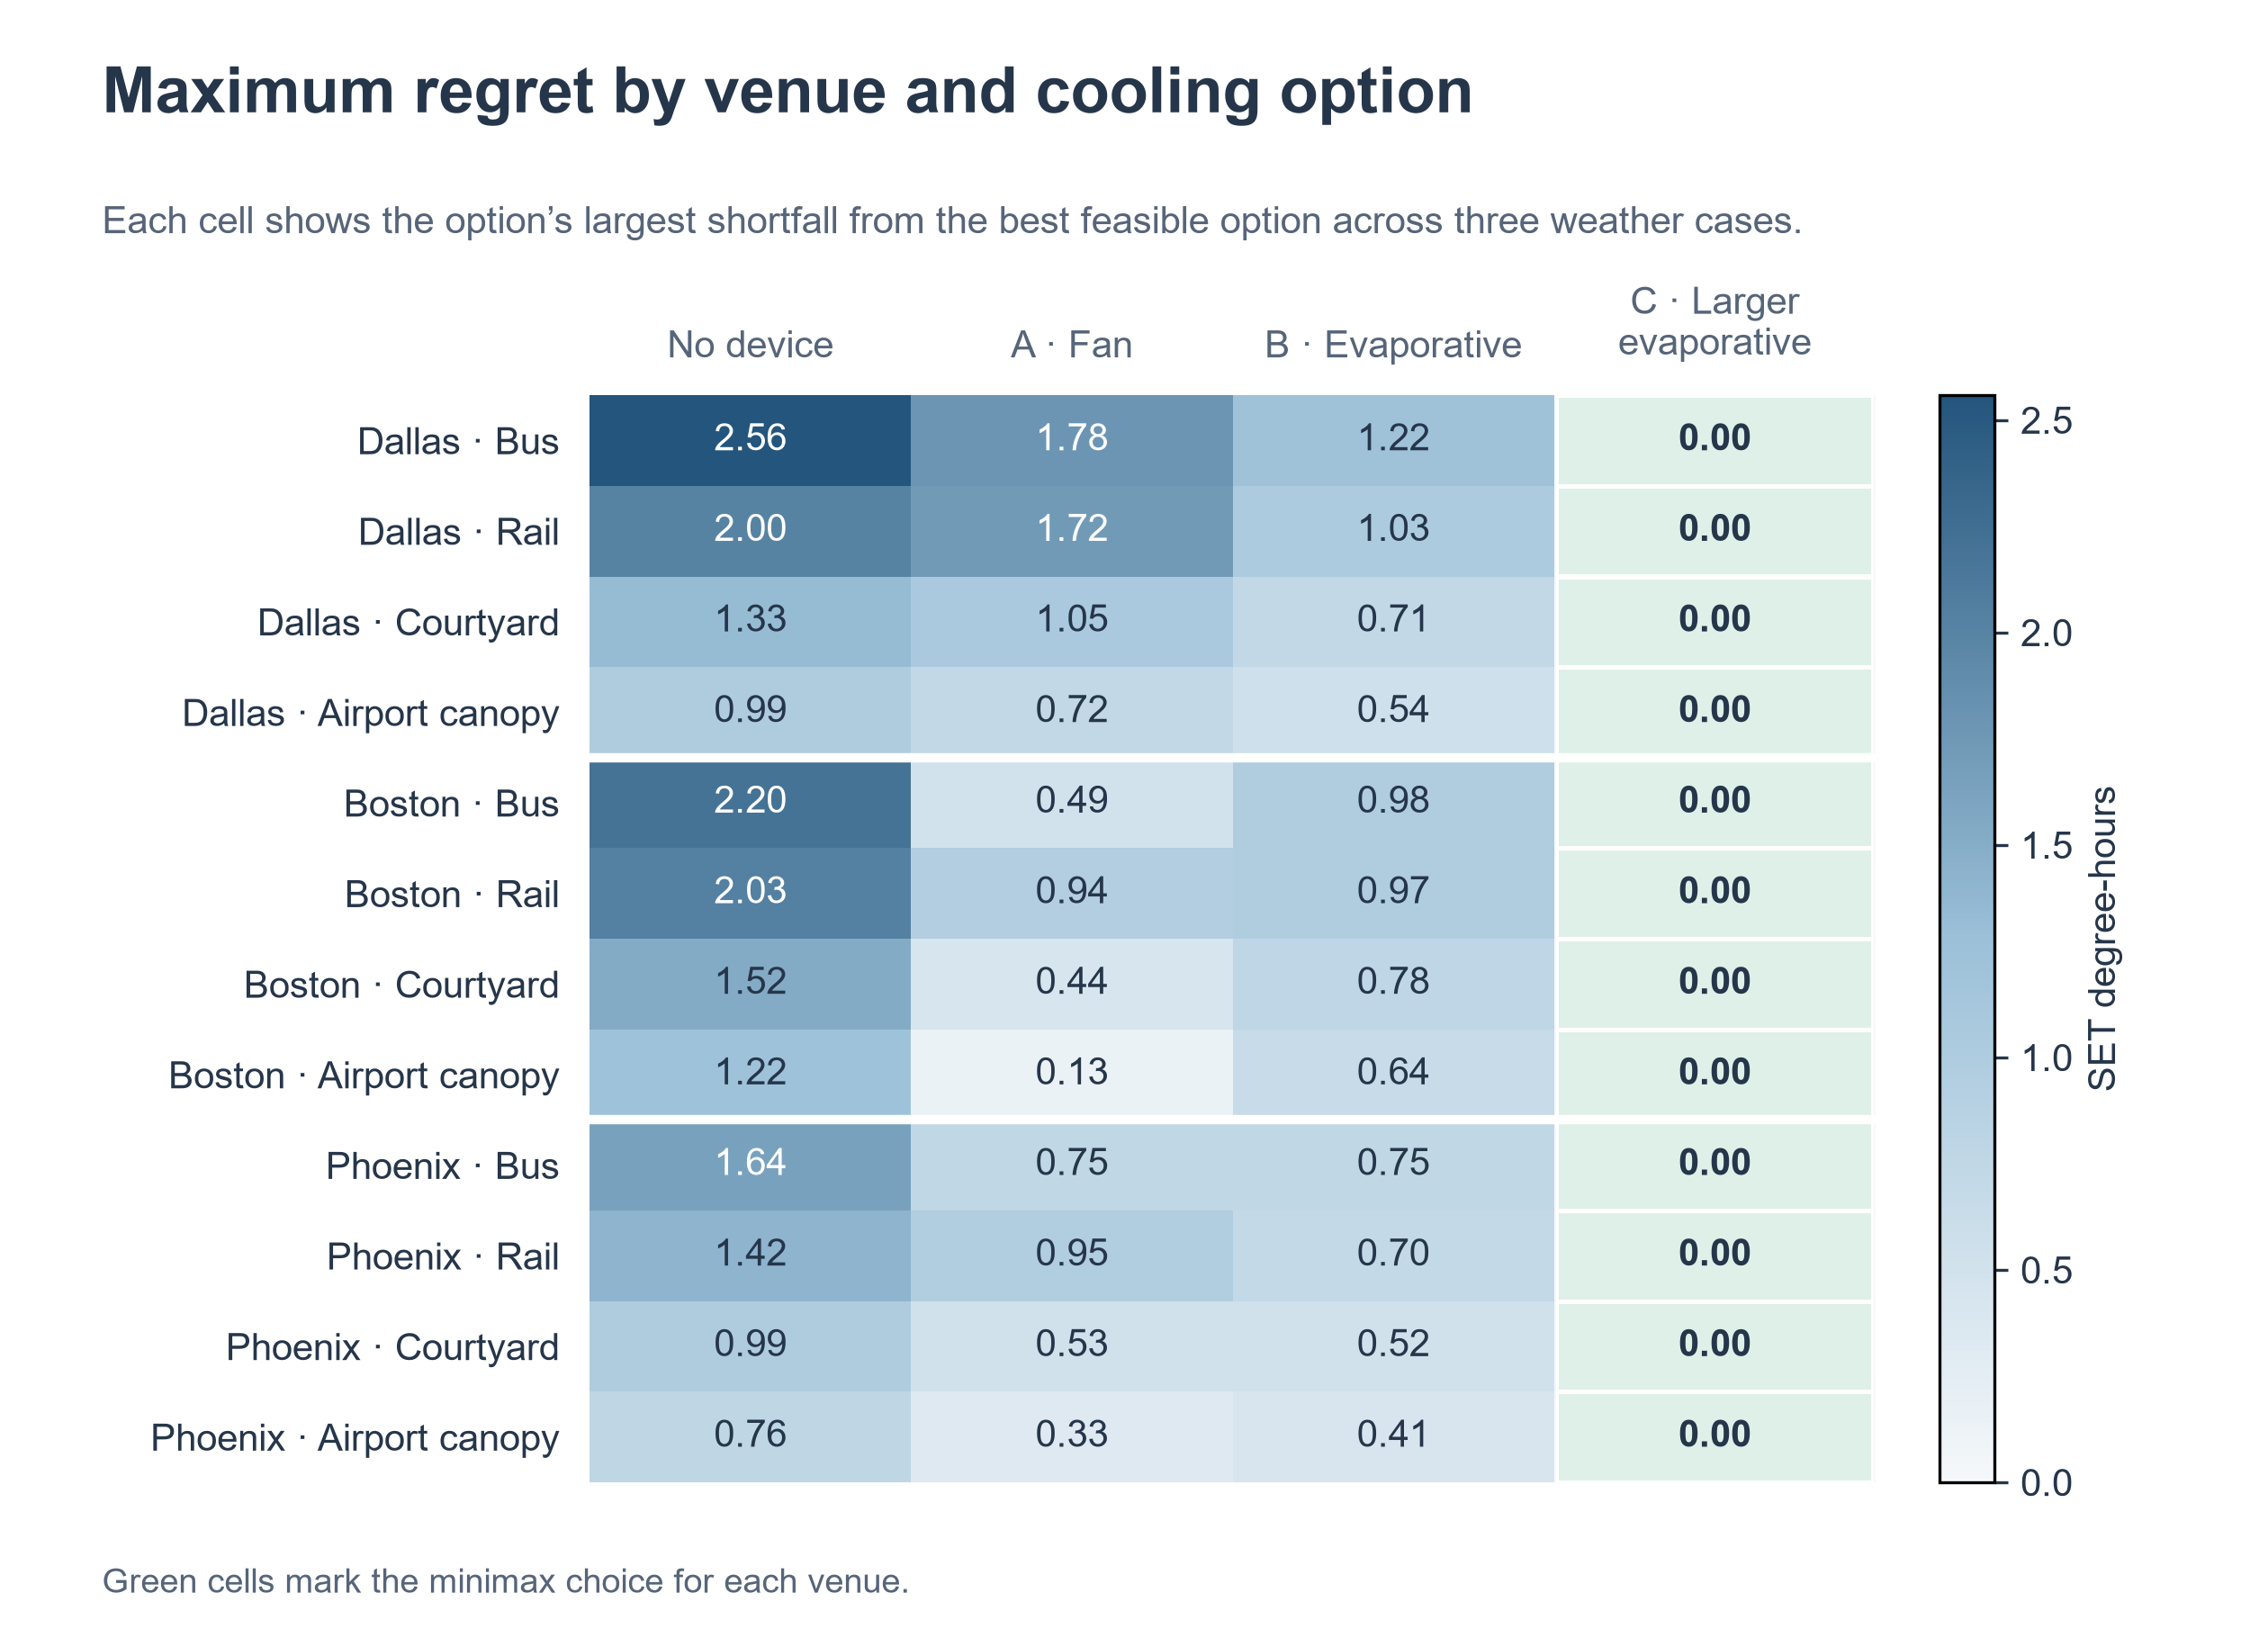
\includegraphics[width=0.88\linewidth]{Images/F7_maximum_regret_all_venues.png}
    \caption{Maximum regret in SET degree-hours across the three modeled scenarios. The green cells identify the minimax recommendation.}
    \label{fig:max-regret}
\end{figure}

At the Dallas bus shelter, maximum regret was 1.78 SET degree-hours for the fan and 1.22 for the smaller cooler. At the Dallas rail platform, the corresponding values were 1.72 and 1.03. The larger cooler had zero maximum regret at both sites.

\subsection{Resource Tradeoffs at Bus Shelters}

The Dallas bus and rail radars share the same axis scales. Both sites use the same equipment and share city weather, so their modeled resource inputs coincide. The different regret profiles reflect how those devices perform under each venue's airflow assumptions.

\begin{figure}[H]
    \centering
    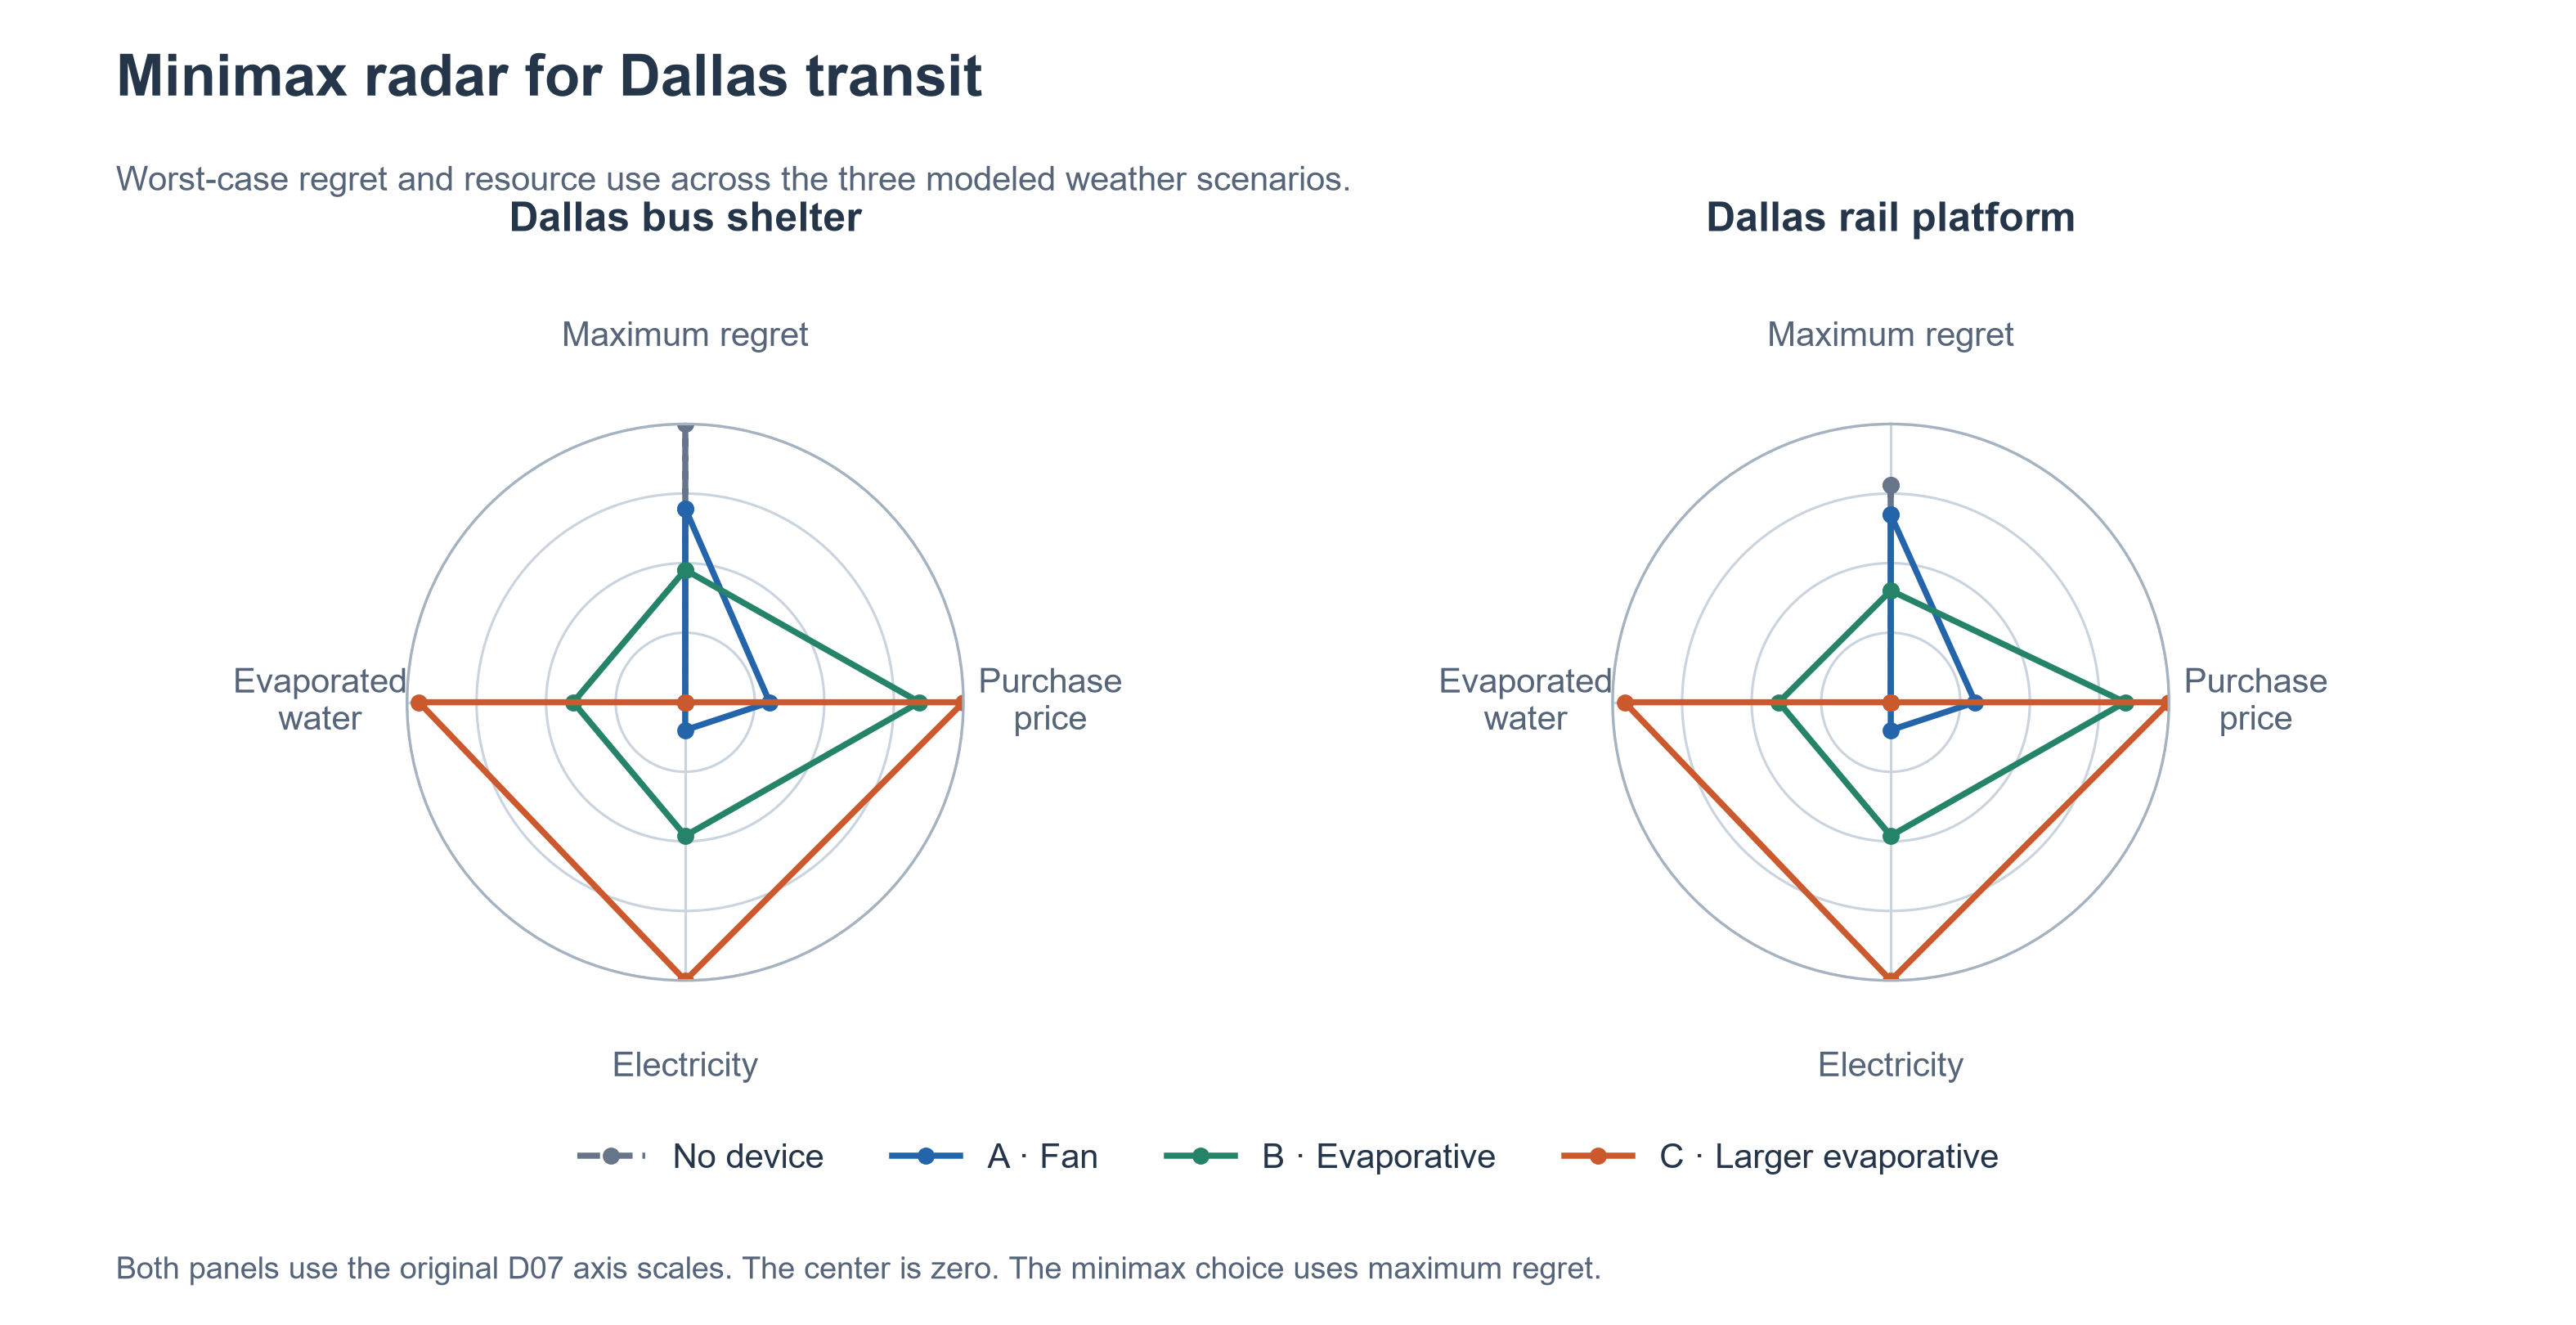
\includegraphics[width=0.94\linewidth]{Images/F15_dallas_transit_minimax_radar.png}
    \caption{Dallas bus shelter and rail platform radars using the generated D07 axis scales. Minimax selection uses the maximum-regret axis.}
    \label{fig:dallas-radar}
\end{figure}

The larger cooler has a recorded reference purchase price of \$4,939~\cite{portacool_4000}. It draws 2.50 kWh over the modeled hour, and evaporates about 44 to 84 kg of water across the 36 modeled cases. Among bus shelters, the smaller cooler is on the cost--regret frontier in Dallas. In Boston and Phoenix, the fan costs less and has lower maximum regret than the smaller cooler.

\begin{figure}[H]
    \centering
    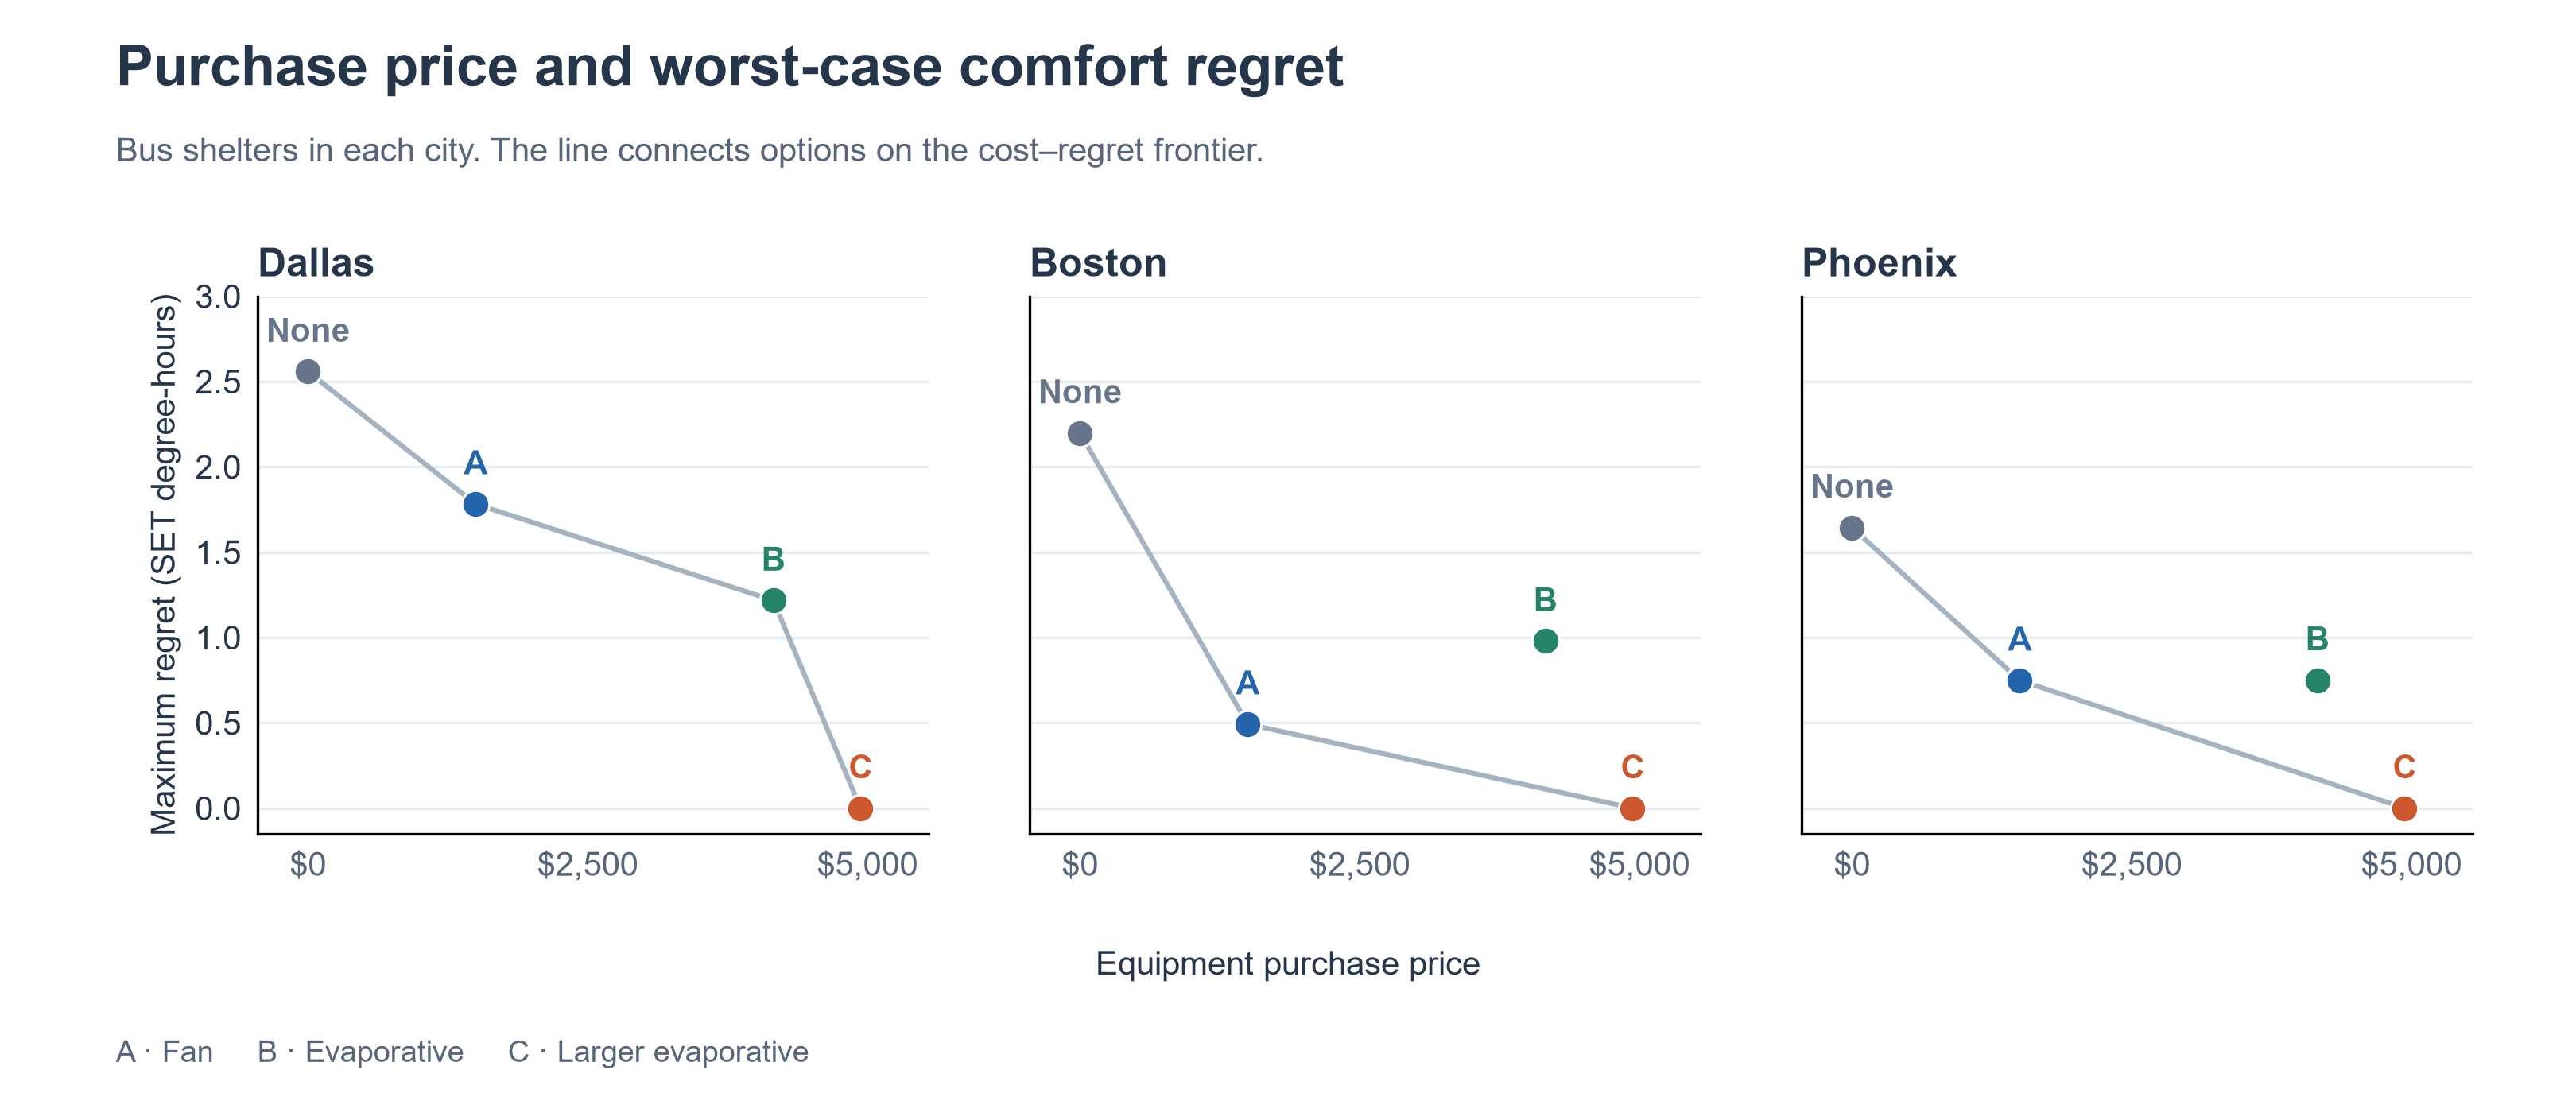
\includegraphics[width=0.92\linewidth]{Images/F13_bus_cost_regret_frontier.png}
    \caption{Purchase price and maximum regret at the three bus shelters. The frontier connects options for which a lower-regret choice costs more.}
    \label{fig:cost-regret}
\end{figure}

\newpage

\subsection{Remaining Discomfort and Sensitivity}

With Option C, peak-hour SET ranged from 28.12\ensuremath{^{\circ}\mathrm{C}} to 33.98\ensuremath{^{\circ}\mathrm{C}} across the 12 venues. Every modeled peak-hour result remained above the 26\ensuremath{^{\circ}\mathrm{C}} comparison target.

\begin{figure}[H]
    \centering
    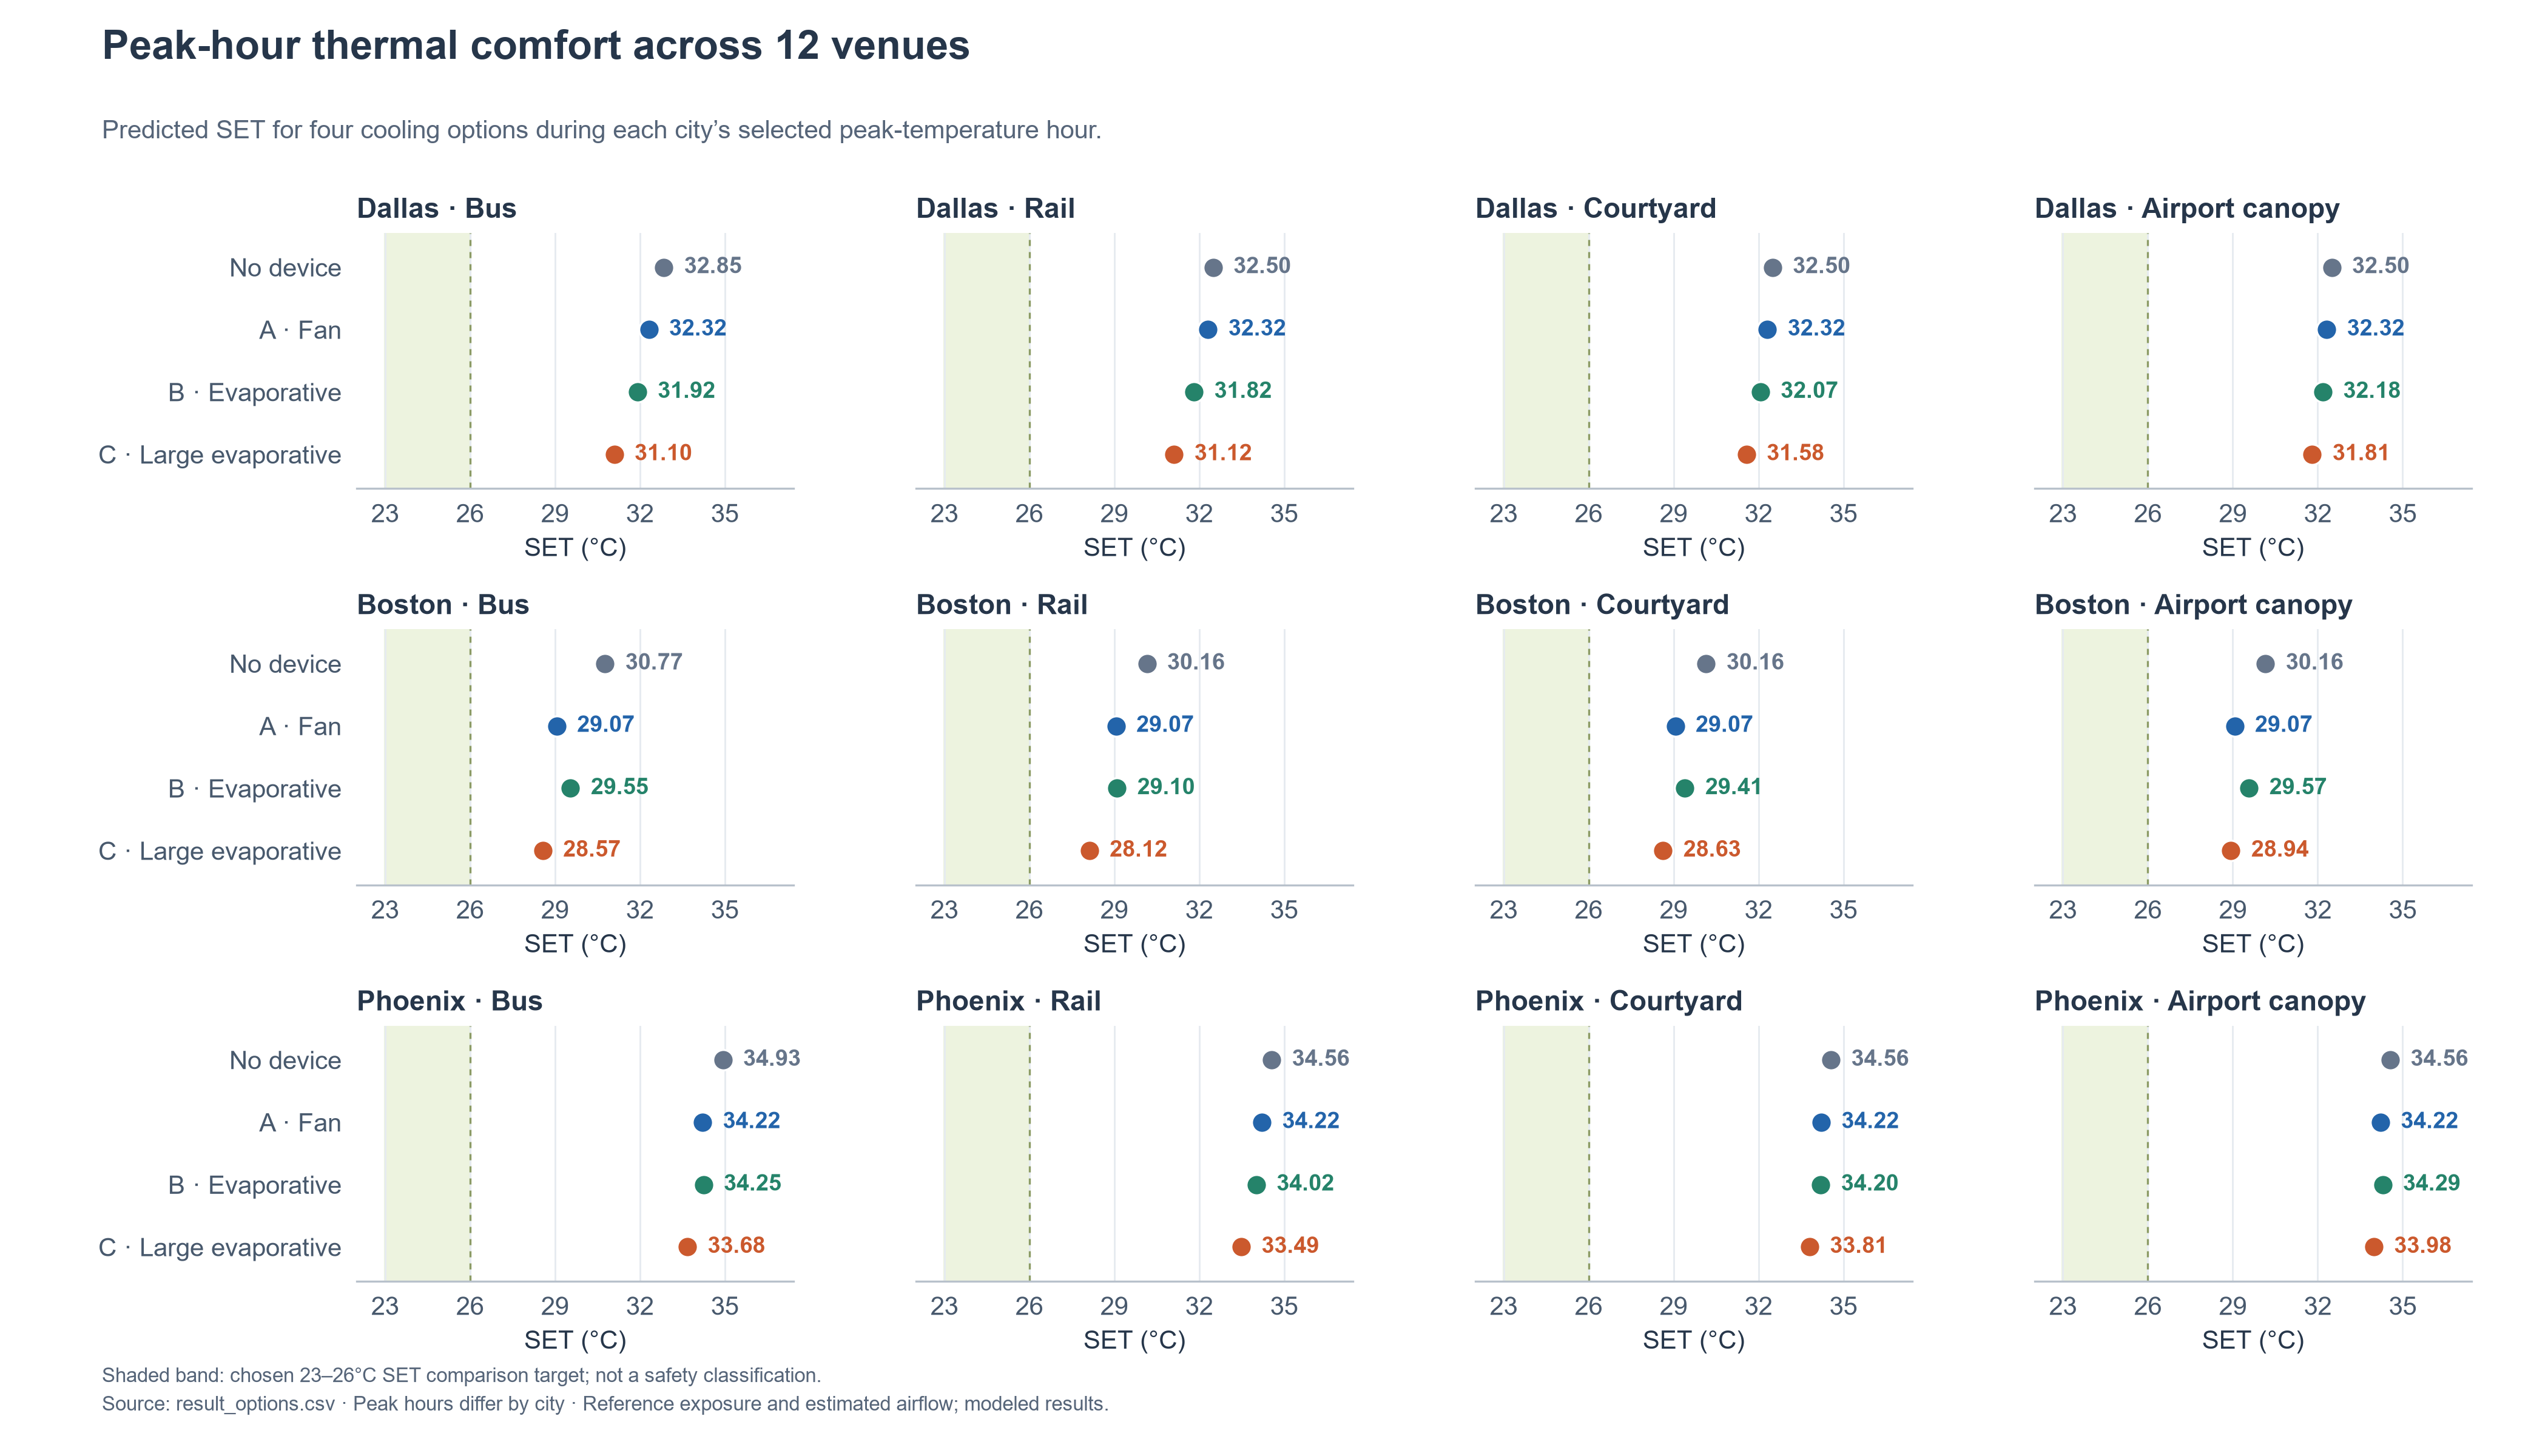
\includegraphics[width=0.95\linewidth]{Images/F3_all_venues_peak_comfort.png}
    \caption{Peak-hour SET at all 12 venues. The shaded band marks the 23--26\ensuremath{^{\circ}\mathrm{C}} comparison target.}
    \label{fig:peak-comfort}
\end{figure}

One-at-a-time sensitivity sweeps identified five intervals where a Boston recommendation changed between the fan and larger cooler. Increasing hot-humid outdoor temperature switched the choice to the fan at the bus stop, courtyard, and airport canopy. Raising the upper SET threshold switched the choice to the larger cooler in two tested intervals.

\begin{figure}[H]
    \centering
    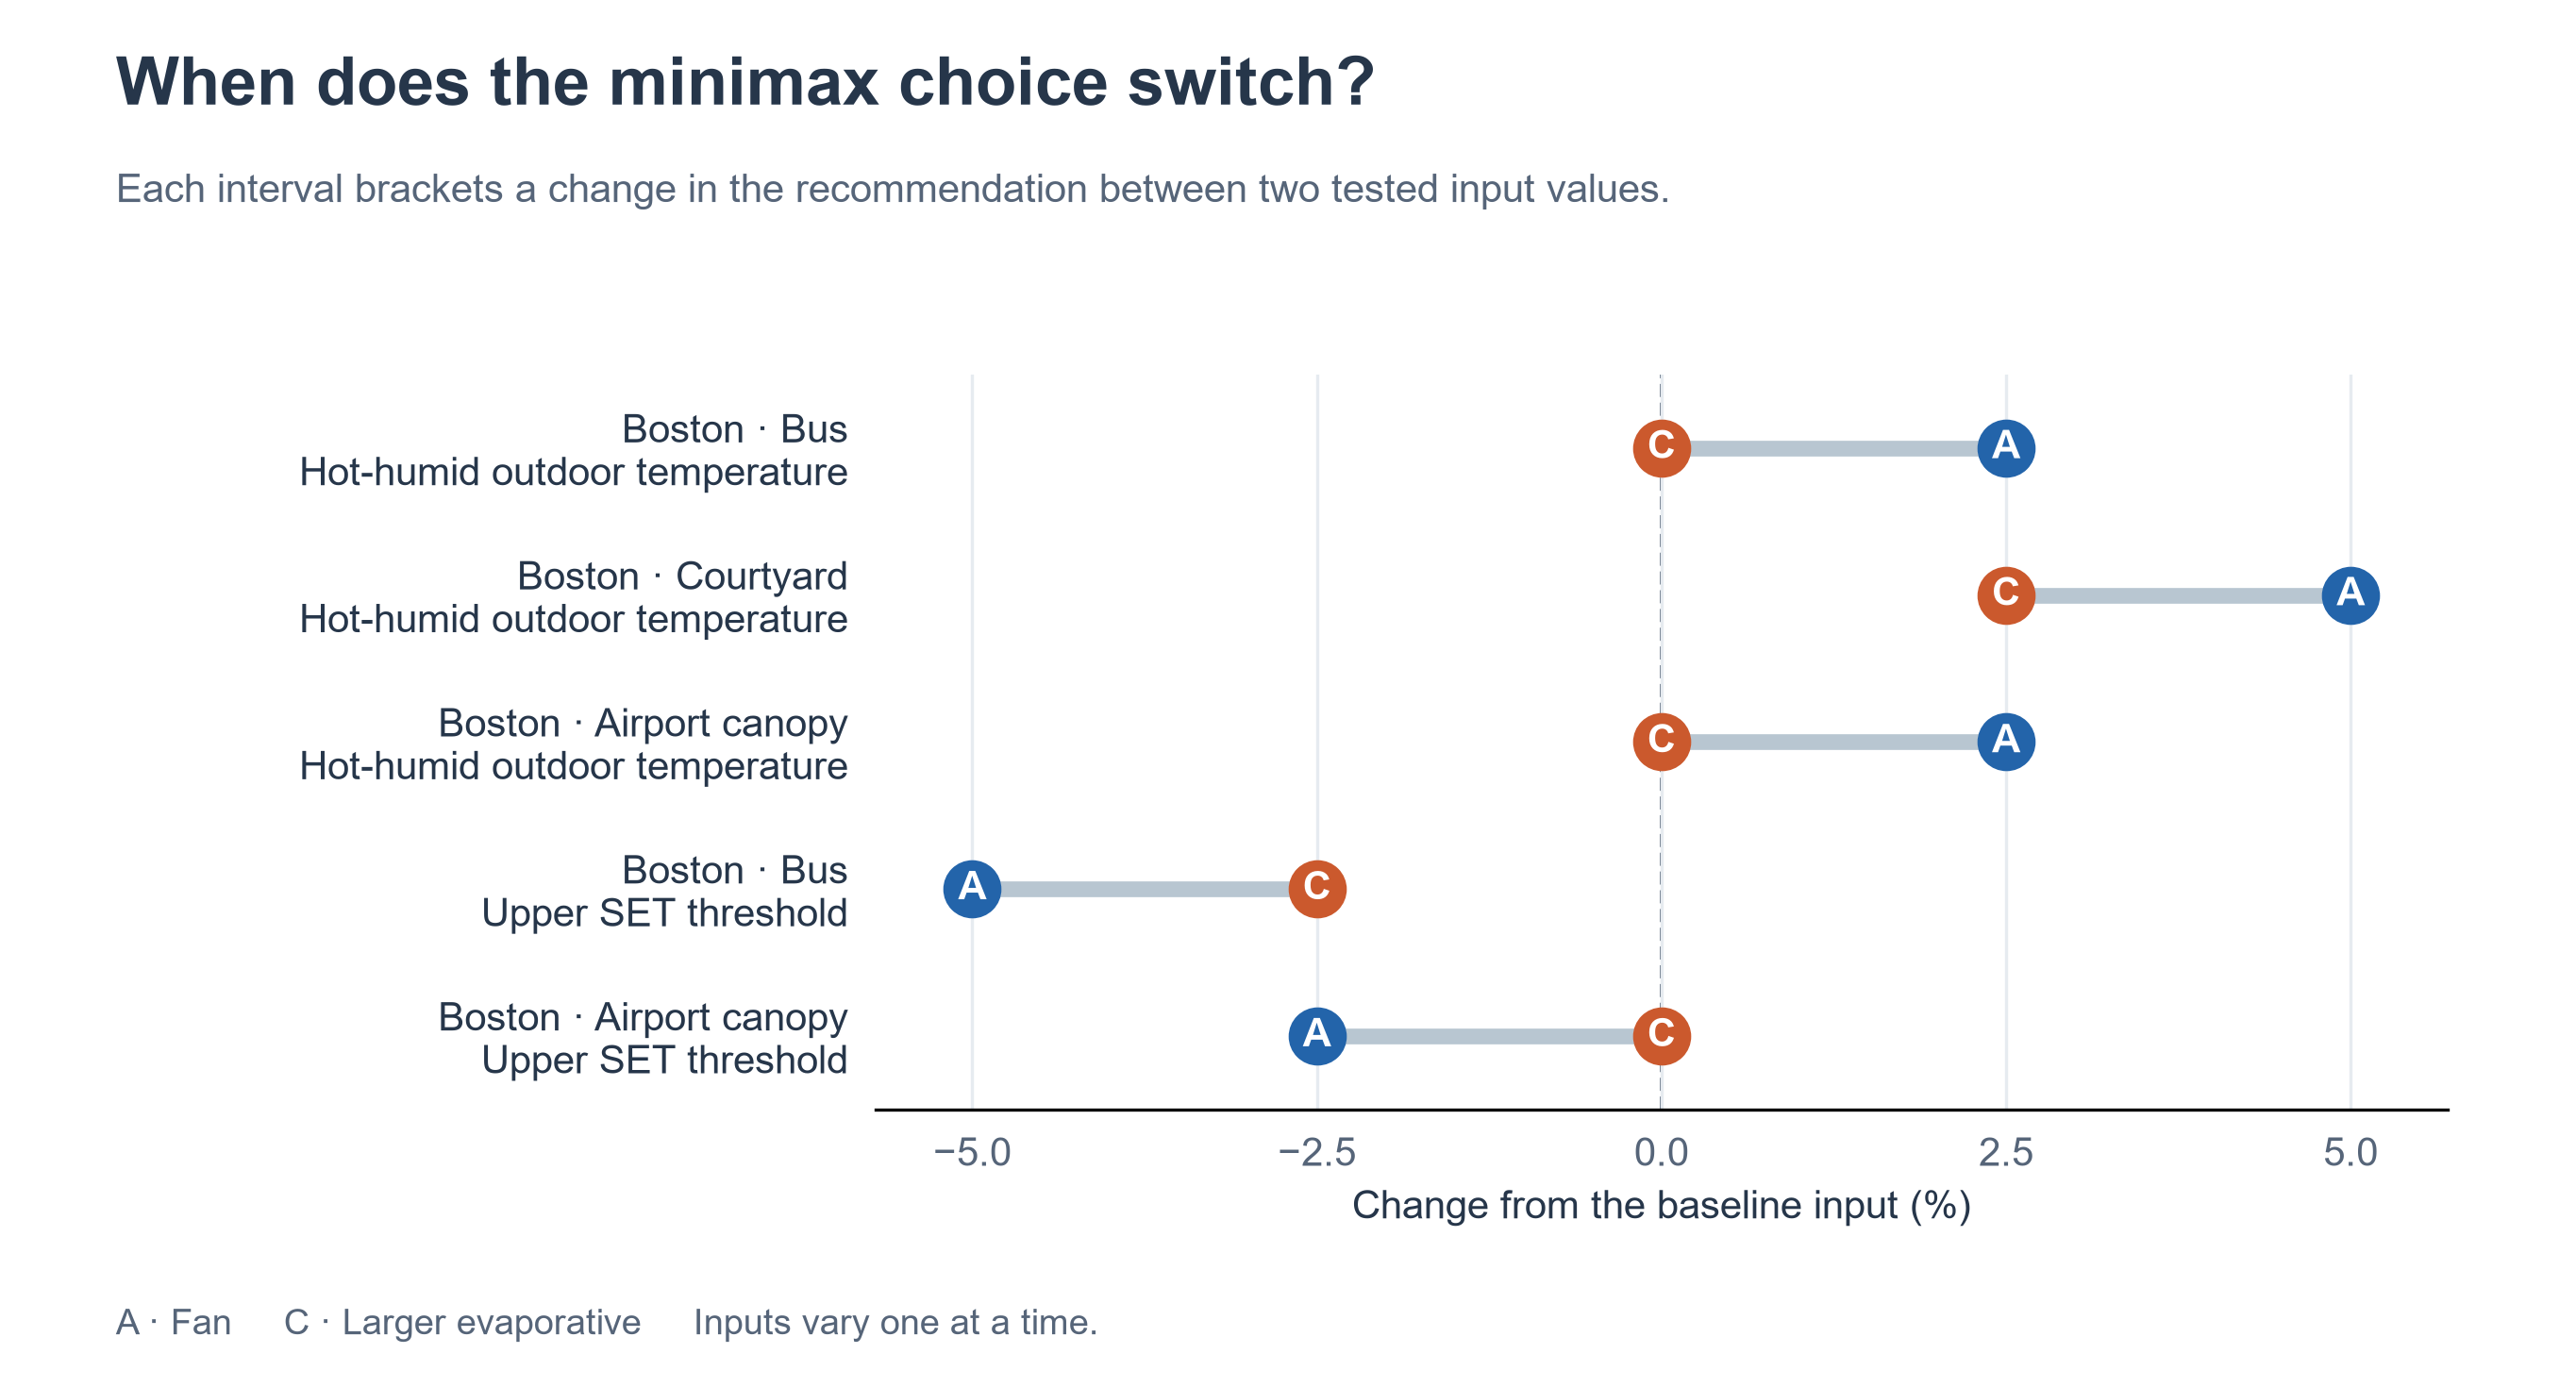
\includegraphics[width=0.78\linewidth]{Images/F14_minimax_sensitivity_switches.png}
    \caption{Tested intervals containing a recommendation change. Endpoints show the selected option at adjacent tested settings. Only the winning option at each endpoint is labeled. Option B was evaluated throughout the sweep.}
    \label{fig:regret-switches}
\end{figure}
